% Copyright © 2012 Martin Ueding <dev@martin-ueding.de>
%
\documentclass[11pt]{article}

\usepackage[a4paper, left=3cm, right=2cm, top=2cm, bottom=2cm]{geometry}
\usepackage[activate]{pdfcprot}
\usepackage[ngerman]{babel}
\usepackage[parfill]{parskip}
\usepackage[T1]{fontenc}
\usepackage[utf8]{inputenc}
\usepackage{amsmath}
\usepackage{amssymb}
\usepackage{amsthm}
\usepackage{color}
\usepackage{epstopdf}
\usepackage{float}
\usepackage{graphicx}
\usepackage{hyperref}
\usepackage{setspace}
\usepackage{units}

\definecolor{darkblue}{rgb}{0,0,.5}

\hypersetup{
	breaklinks=false,
	colorlinks=true,
	linkcolor=black,
	menucolor=black,
	urlcolor=darkblue
}

\setlength{\columnsep}{2cm}

\DeclareMathOperator{\arcsinh}{arsinh}
\DeclareMathOperator{\arsinh}{arsinh}
\DeclareMathOperator{\asinh}{arsinh}
\DeclareMathOperator{\card}{card}
\DeclareMathOperator{\diam}{diam}

\newcommand{\emesswert}{\left(\messwert \pm \messwert \right)}
\newcommand{\e}[1]{\cdot 10^{#1}}
\newcommand{\fehlt}{\textcolor{red}{Hier fehlen noch Inhalte.}}
\newcommand{\half}{\frac{1}{2}}
\newcommand{\laplace}{\vnabla^2}
\newcommand{\messwert}{\textcolor{blue}{\square}}
\newcommand{\vnabla}{\vec{\nabla}}

\renewcommand{\d}{\, \mathrm d}

\title{physik212 -- Versuch 249 \\ Elektrische und magnetische Kraftwirkung auf geladene Teilchen}
\author{Martin Ueding \\ \href{mailto:mu@uni-bonn.de}{mu@uni-bonn.de}}

\begin{document}

\maketitle

\tableofcontents

\vfill

Stellen in \textcolor{blue}{blau} werden bei der Versuchsdurchführung
eingetragen. Zum Beispiel werden Messwerte mit „$\messwert$“ markiert. Stellen
in \textcolor{red}{rot} müssen noch vor Versuchsbeginn vervollständigt werden.

\newpage

%%%%%%%%%%%%%%%%%%%%%%%%%%%%%%%%%%%%%%%%%%%%%%%%%%%%%%%%%%%%%%%%%%%%%%%%%%%%%%%
%                                 Einleitung                                  %
%%%%%%%%%%%%%%%%%%%%%%%%%%%%%%%%%%%%%%%%%%%%%%%%%%%%%%%%%%%%%%%%%%%%%%%%%%%%%%%

\section{Einleitung}

In diesen Versuchen wollen wir die Ladung und Masse des Elektrons bestimmen.
Dazu bestimmen wir zuerst die spezifische Masse $\frac em$ mit dem
Fadenstrahlrohr und anschließend die Ladung $e$ mit dem Millikanversuch.

%%%%%%%%%%%%%%%%%%%%%%%%%%%%%%%%%%%%%%%%%%%%%%%%%%%%%%%%%%%%%%%%%%%%%%%%%%%%%%%
%                                   Theorie                                   %
%%%%%%%%%%%%%%%%%%%%%%%%%%%%%%%%%%%%%%%%%%%%%%%%%%%%%%%%%%%%%%%%%%%%%%%%%%%%%%%

\section{Theorie}

\subsection{Fadenstrahlrohr}

Im Fadenstrahlrohr werden Elektronen auf eine Energie $W = Ue$ beschleunigt.
Damit haben sie eine Geschwindigkeit von $v = \sqrt{\frac{2W}{m}}$. Im
Magnetfeld $B$ beschreiben sie eine Kreisbahn mit:
\[ m \frac{v^2}r = e v B \]

Daraus kann man die spezifische Masse ableiten:
\begin{equation}
	\label{eq:spezifische-Masse}
	\frac em = \frac{2U}{r^2 B^2}
\end{equation}

Das Magnetfeld im Inneren der Helmholtz-Spulen kann nach Biot-Savart
hergeleitet werden und ist gegeben durch:
\begin{equation}
	\label{eq:Helmholtz}
	B = 0.716 \mu_0 \frac{nI}R
\end{equation}

\subsection{Millikanversuch}

Im Millikanversuch werden einzelne Öltröpfchen, die wenige Elementarladungen
tragen, in einen Kondensator gebracht. Ihr Radius wird über die
Sedimentgeschwindigkeiten bestimmt.
%
\begin{equation}
	\label{eq:249.8}
	r = \sqrt{\frac{9 \eta \left( v_\Downarrow - v_\Uparrow \right)}{4 g (\rho_\text{Öl} - \rho_\text{Luft})}}
\end{equation}

Über die Dichte wird dann die Masse bestimmt, daraus dann die
Schwerebeschleunigung. Daraus kann dann die elektrische Kraft bestimmt werden,
woraus die Ladung folgt.
%
\begin{equation}
	\label{eq:249.9}
	N e = 3 \pi \eta r \frac{v_\Downarrow + v_\Uparrow }E
\end{equation}

%%%%%%%%%%%%%%%%%%%%%%%%%%%%%%%%%%%%%%%%%%%%%%%%%%%%%%%%%%%%%%%%%%%%%%%%%%%%%%%
%                                  Aufgaben                                   %
%%%%%%%%%%%%%%%%%%%%%%%%%%%%%%%%%%%%%%%%%%%%%%%%%%%%%%%%%%%%%%%%%%%%%%%%%%%%%%%

\section{Aufgaben}

\subsection{Aufgabe A: Skizzen}

Es sollen die Kraftvektoren skizziert werden. Dies habe ich für ein
aufsteigendes Öltröpfchen in Abbildung \ref{fig:aufsteigend} und für fallendes
in Abbildung \ref{fig:fallend} gemacht.

\begin{figure}[h!]
	\centering
	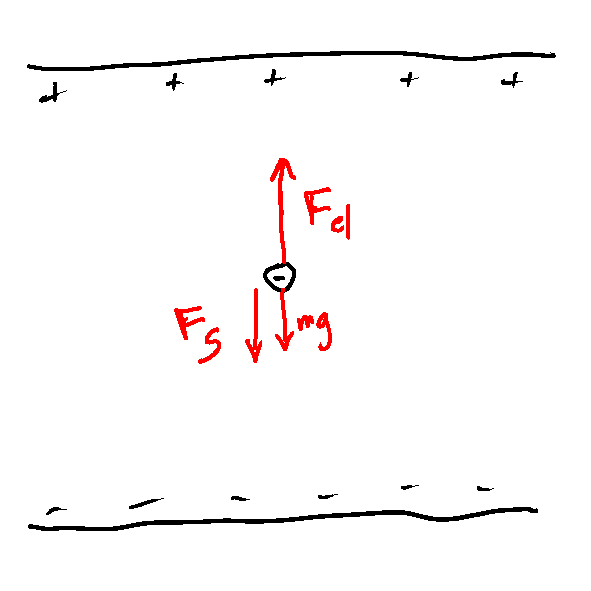
\includegraphics[width=.5\textwidth]{aufsteigend.pdf}
	\caption{aufsteigendes Öltröpfchen}
	\label{fig:aufsteigend}
\end{figure}

\begin{figure}[h!]
	\centering
	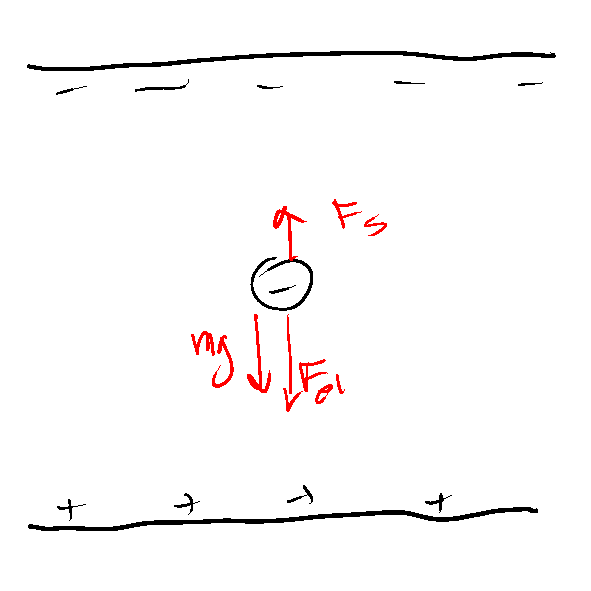
\includegraphics[width=.5\textwidth]{fallend.pdf}
	\caption{fallendes Öltröpfchen}
	\label{fig:fallend}
\end{figure}

\subsection{Aufgabe B: Gleichung 249.10}

Es soll die Gleichung 249.10 bewiesen werden:
\begin{equation}
	\label{eq:249.10}
	2 v_\circ = v_\Downarrow - v_\Uparrow
\end{equation}

\begin{proof}
	In der Anleitung sind folgende Formeln gegeben. Sie beschreiben das
	Kräftegleichgewicht für ein fallendes \eqref{eq:A-fallend} und steigendes
	\eqref{eq:A-steigend} Tröpfchen:
	%
	\begin{equation}
		\label{eq:A-fallend}
		\frac{4 \pi}3 r^3 \left( \rho_\text{Öl} - \rho_\text{Luft} \right) g
		- 6 \pi \eta r v_\Downarrow
		= - N e E
	\end{equation}
	%
	\begin{equation}
		\label{eq:A-steigend}
		\frac{4 \pi}3 r^3 \left( \rho_\text{Öl} - \rho_\text{Luft} \right) g
		+ 6 \pi \eta r v_\Uparrow
		= + N e E
	\end{equation}

	Entsprechend kann ich auch ein Kräftegleichgewicht für ein fehlendes
	elektrisches Feld aufstellen:
	%
	\begin{equation}
		\label{eq:A-alleine}
		\frac{4 \pi}3 r^3 \left( \rho_\text{Öl} - \rho_\text{Luft} \right) g
		+ 6 \pi \eta r v_\circ
		= 0
	\end{equation}

	Nun rechne ich $2 \eqref{eq:A-alleine} - \eqref{eq:A-fallend} -
	\eqref{eq:A-steigend}$, so dass sich der Teil der Schwerkraft und des
	elektrischen Felds weghebt und erhalte:
	%
	\begin{align*}
		12 \pi \eta r v_\circ - 6 \pi \eta r v_\Downarrow + 6 \pi \eta r v_\Uparrow &= 0 \\
		2 v_\circ - v_\Downarrow + v_\Uparrow &= 0 \\
		2 v_\circ &= v_\Downarrow - v_\Uparrow \\
	\end{align*}

	Dies ist die gesuchte Beziehung.
\end{proof}

\subsection{Aufgabe C: Gleichung 249.11}

Es soll die Gleichung 249.11 bewiesen werden:
\[ e_\circ = e_{S, i} \left( 1 + \frac A{r_i} \right)^{-\frac 32} \]

\begin{proof}
	In Gleichung \eqref{eq:249.8} ist zu sehen, dass gilt:
	\[ r \propto \eta^{\frac 12} \]

	In Gleichung \eqref{eq:249.9} taucht noch ein $\eta$ neben dem $r$ auf.
	Somit gilt also:
	\[ N e \propto \eta^{\frac 32} \]

	Im Text wurde erwähnt, dass gilt:
	\[ \eta_\text{eff} = \eta_\text{Luft} \left( 1 + \frac Ar \right)^{-1} \]

	Somit gilt:
	\[ e_\circ = e_S \left( 1 + \frac Ar \right)^{-\frac 32} \]
\end{proof}

%%%%%%%%%%%%%%%%%%%%%%%%%%%%%%%%%%%%%%%%%%%%%%%%%%%%%%%%%%%%%%%%%%%%%%%%%%%%%%%
%                          Aufbau und Durchführung                            %
%%%%%%%%%%%%%%%%%%%%%%%%%%%%%%%%%%%%%%%%%%%%%%%%%%%%%%%%%%%%%%%%%%%%%%%%%%%%%%%

\section{Aufbau und Durchführung}

\subsection{Fadenstrahlrohr}

Wir beginnen mit dem Fadenstrahlrohr. Der Aufbau ist in Abbildung
\ref{fig:Fadenstrahlrohr} skizziert. Dieses besteht aus einer Elektronenkanone,
die mit Beschleunigungsgitter und Wehnelt-Zylinder die Elektronen vom Heizdraht
zu einem dünnen Strahl beschleunigt. Die Elektronen bewegen sich in einem
Magnetfeld, das senkrecht zu ihrer Bewegungsrichtung steht. Das Feld wird zur
ein Helmholtz-Spulenpaar erzeugt.

\begin{figure}[h!]
	\centering
	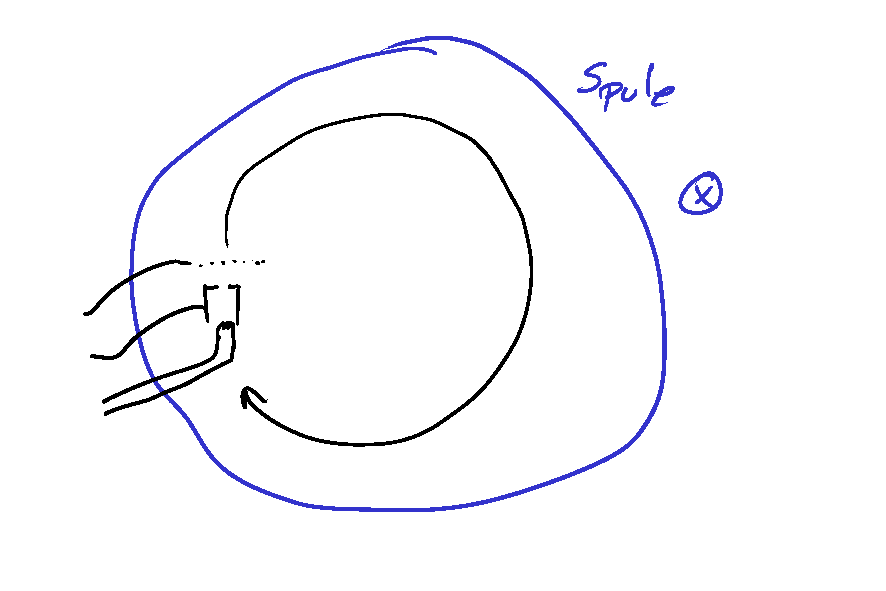
\includegraphics[width=\textwidth]{Aufbau_Fadenstrahlrohr.pdf}
	\caption{Zeichnung des Aufbaus für den ersten Versuchsteil mit dem Fadenstrahlrohr.}
	\label{fig:Fadenstrahlrohr}
\end{figure}

\subsubsection{Aufgabe a: Fadenstrahlrohr}

\label{Durchführung-a}

Wir heizen das Fadenstrahlrohr ungefähr drei Minuten auf. Danach wählen wir
eine Spannung für Anode $U_A$ und Wehnelt-Zylinder $U_W$. Deren Differenz ist
die Beschleunigungsspannung $U$. Diese bestimme ich allerdings erst in der
Auswertung.

Dann leuchten wir die Messeinrichtung im Inneren mit einer Taschenlampe an,
damit diese phosphoresziert. Wir schalten den Strom durch die Helmholtz-Spulen
ein. Damit der Fadenstrahl genau senkrecht zum Magnetfeld verläuft, drehen wir
das Fadenstrahlrohr entsprechend.

Nun stellen wir den Spulenstrom so ein, dass der Strahl genau auf eine
Messmarke trifft. Wir lesen die Beschleunigungsspannung $U$, den Radius $r$ und
den Spulenstrom $I$ ab.

Wir wiederholen diesen Messvorgang einige Male mit verschiedenen $U$ und $I$
für alle Radien. Für jede Spannung und jeden Radius messen wir zweimal. Einmal
den Elektronenstrahl nach oben und einmal nach unten (der Strom wird umgepolt).
Den Strom regeln wir dann so, dass der Radius wieder eingehalten wird.

Die Messwerte sind in Tabelle \ref{table:Aufgabe-a}.

\begin{table}[H]
	\centering

	\begin{tabular}{cccc}
		$r$ in $\unit m$ & $U$ in $\unit V$ & $I_1$ in $\unit A$ & $I_2$ in $\unit A$ \\
		\hline
		$0.02$ & $\messwert$ & $\messwert$ & $\messwert$ \\
		$0.03$ & $\messwert$ & $\messwert$ & $\messwert$ \\
		$0.04$ & $\messwert$ & $\messwert$ & $\messwert$ \\
		$0.05$ & $\messwert$ & $\messwert$ & $\messwert$ \\
		\hline
		$0.02$ & $\messwert$ & $\messwert$ & $\messwert$ \\
		$0.03$ & $\messwert$ & $\messwert$ & $\messwert$ \\
		$0.04$ & $\messwert$ & $\messwert$ & $\messwert$ \\
		$0.05$ & $\messwert$ & $\messwert$ & $\messwert$ \\
		\hline
		$0.02$ & $\messwert$ & $\messwert$ & $\messwert$ \\
		$0.03$ & $\messwert$ & $\messwert$ & $\messwert$ \\
		$0.04$ & $\messwert$ & $\messwert$ & $\messwert$ \\
		$0.05$ & $\messwert$ & $\messwert$ & $\messwert$ \\
		\hline
		   \vdots & \vdots & \vdots
	\end{tabular}

	\caption{Messwerte aus Aufgabe a}
	\label{table:Aufgabe-a}
\end{table}

Dabei sind die Fehler für die Messwerte:
\[
	\Delta U = \unit[\messwert] V,
	\quad
	\Delta r = \unit[\messwert] m,
	\quad
	\Delta I = \unit[\messwert] A
\]

Diese Daten werte ich in \ref{Auswertung-b} aus.

\subsection{Millikanversuch}

Im zweiten Teil benutzen wir eine kommerzielle Millikan-Apparatur. In dieser
werden geladene Öltröpfchen zwischen zwei Kondensatorplatten gesprüht. Die
Tröpfchen tragen einige wenige Elementarladungen und wechselwirken so mit dem
elektrischen Feld im Kondensator.

Mit einem Mikroskop können wir die Bewegung der Teilchen beobachten.

\begin{figure}[h!]
	\centering
	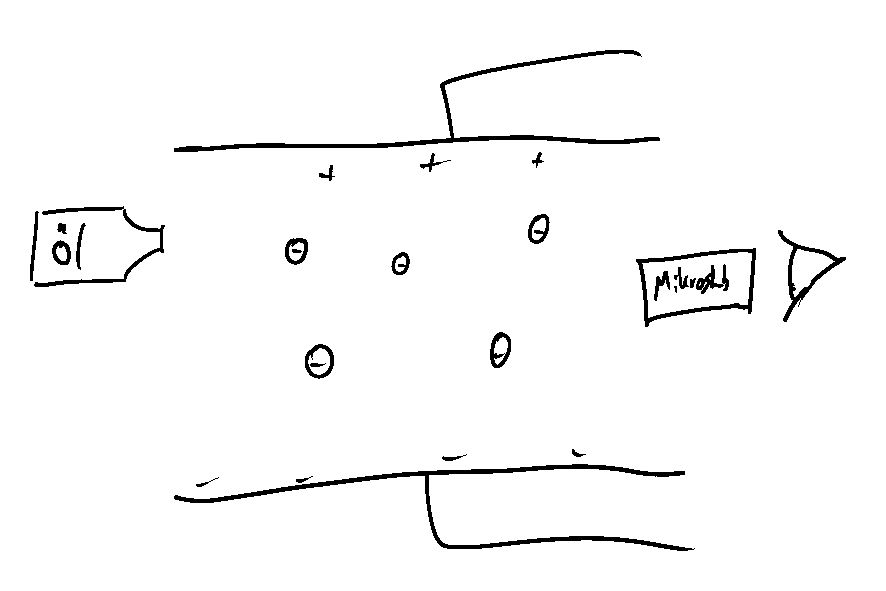
\includegraphics[width=\textwidth]{Aufbau_Millikanversuch.pdf}
	\caption{Zeichnung des Aufbaus für den zweiten Versuchsteil mit dem
	Millikanversuch.}
	\label{fig:Millikanversuch}
\end{figure}

\subsubsection{Aufgabe c: Tröpfchen sprühen}

Wir testen den Zerstäuber an einem Blatt Papier. Wenn wir am Papier Öl sehen,
funktioniert dieser und wir können ihn in der Apparatur benutzen.

Anschließend sprühen wir einmal Öl zwischen die Kondensatorplatten, die zu
diesem Zeitpunkt geerdet sein müssen. Sobald wir Tröpfchen erkennen können,
schließen wir das Entlüftungsloch sowie das Eintrittsloch.

\subsubsection{Aufgabe d: Tröpfchenauswahl}

Wir suchen ein Öltröpfchen aus, das wir beobachten wollen. Durch Einschalten
des elektrischen Feldes können wir geladene Teilchen finden. Falls sich diese
zu schnell bewegen oder zu klein sind, müssen wir diese verwerfen. Eventuell
benutzen wir die radioaktive Quelle zum Ionisieren.

\subsubsection{Aufgabe e: Sedimentgeschwindigkeiten}

Für ein bestimmtes Teilchen messen wir die Sedimentgeschwindigkeiten, einmal
mit Feld, einmal mit umgepolten Feld und einmal ohne Feld. Dazu stoppen wir die
Zeit und zählen die Anzahl Striche, die das Tröpfchen zurücklegt im Mikroskop.

\subsubsection{Aufgabe f: weitere Tröpfchen}

Wir messen für mindestens 10 Tröpfchen die drei Sedimentgeschwindigkeiten fünf
Mal. Dabei messen wir immer eine Strecke und eine Zeit. Die Daten sind in
Tabelle \ref{table:sediment1}.

Die Messfehler ergeben sich später in \ref{Auswertung-f} aus der Statistik, da
ja jedes Tröpfchen fünf Mal vermessen wird. Wir schätzen diese an dieser Stelle
auf:
\[
	\Delta s = \unit[\messwert] m
	, \quad
	\Delta t = \unit[\messwert] s
\]

\begin{table}[h!]
	\centering

	\begin{tabular}{cccccc}
		$s_\circ$ in $\unit m$ & $t_\circ$ in $\unit s$ & $s_\Downarrow$ in $\unit m$ & $t_\Downarrow$ in $\unit s$ & $s_\Uparrow$ in $\unit m$ & $t_\Uparrow$ in $\unit s$ \\
		\hline \hline
		$\messwert$ & $\messwert$ & $\messwert$ & $\messwert$ & $\messwert$ & $\messwert$\\
		$\messwert$ & $\messwert$ & $\messwert$ & $\messwert$ & $\messwert$ & $\messwert$\\
		$\messwert$ & $\messwert$ & $\messwert$ & $\messwert$ & $\messwert$ & $\messwert$\\
		$\messwert$ & $\messwert$ & $\messwert$ & $\messwert$ & $\messwert$ & $\messwert$\\
		$\messwert$ & $\messwert$ & $\messwert$ & $\messwert$ & $\messwert$ & $\messwert$\\
		\hline
		$\messwert$ & $\messwert$ & $\messwert$ & $\messwert$ & $\messwert$ & $\messwert$\\
		$\messwert$ & $\messwert$ & $\messwert$ & $\messwert$ & $\messwert$ & $\messwert$\\
		$\messwert$ & $\messwert$ & $\messwert$ & $\messwert$ & $\messwert$ & $\messwert$\\
		$\messwert$ & $\messwert$ & $\messwert$ & $\messwert$ & $\messwert$ & $\messwert$\\
		$\messwert$ & $\messwert$ & $\messwert$ & $\messwert$ & $\messwert$ & $\messwert$\\
		\hline
				\vdots & \vdots & \vdots & \vdots & \vdots & \vdots
	\end{tabular}

	\caption{Sedimentgeschwindigkeiten der Öltröpfchen}
	\label{table:sediment1}
\end{table}

Die tatsächlichen Geschwindigkeiten rechne ich in \ref{Auswertung-f} aus.

Wir bestimmen noch die Zimmertemperatur auf:
\[ T = \unit[\emesswert]{^\circ C} \]

%%%%%%%%%%%%%%%%%%%%%%%%%%%%%%%%%%%%%%%%%%%%%%%%%%%%%%%%%%%%%%%%%%%%%%%%%%%%%%%
%                                 Auswertung                                  %
%%%%%%%%%%%%%%%%%%%%%%%%%%%%%%%%%%%%%%%%%%%%%%%%%%%%%%%%%%%%%%%%%%%%%%%%%%%%%%%

\section{Auswertung}

Das GNU Octave Programm, das ich für die Auswertung geschrieben habe, ist unter
\url{http://uni-bonn.de/~s6mauedi/physik212/249.html} zu finden.

\subsection{Aufgabe b: Magnetfelder und spezifische Masse}

\label{Auswertung-b}

Hier werte ich die Daten aus \ref{Durchführung-a} aus.

Die Formel 249.1 aus der Anleitung ist:
\begin{equation}
	\label{eq:249.1}
	\vec F = e \left( \vec v \times \vec B \right)
\end{equation}

Diese soll nun um das Erdmagnetfeld erweitert werden. Somit wird aus
\eqref{eq:249.1}:
\begin{equation}
	\label{eq:Erdmagnetfeld}
	\vec F = e \left( \vec v \times \left( \vec B_S + \vec B_E \right) \right)
\end{equation}

Da allerdings darauf geachtet worden ist, dass überall $\vec v \perp \vec B$
gilt, vereinfacht sich \eqref{eq:Erdmagnetfeld} zu:
\begin{equation}
	\label{eq:magnetische-Kraft}
	F = e v (B_S + B_E)
\end{equation}

Die Magnetfeldstärke der Spulen ist hier nur eine Funktion des Stromes, da
Windungszahl und Widerstand konstant bleibt. Diese Funktion $B_S(I)$ ist in
\eqref{eq:Helmholtz} gegeben.

Der Radius ist in beiden Messungen gleich. Also muss die Kraft und somit das
Magnetfeld gleich sein. Das Erdmagnetfeld sei in Richtung von der ersten
Messung positiv. Somit muss ich es von der zweiten Messung abziehen.
%
\begin{align*}
	F_1 &= F_2 \\
	B_S(I_1) + B_E &= B_S(I_2) - B_E \\
	B_S(I_1) - B_S(I_2) &= - 2 B_E \\
	\intertext{Da $B_S$ linear in $I$ ist, kann ich dies umformen zu:}
	\half B_S(I_2 - I_1) &= B_E \\
\end{align*}

Somit kann ich das Magnetfeld im Inneren durch die beiden Ströme ausdrücken:
\begin{align*}
	B &= B_S(I_1) + \half B_S(I_2 - I_1) \\
	\intertext{Nun wende ich noch mal die Linearität an:}
	B &= B_S \left( \half I_1 + \half I_2 \right) \\
	\intertext{Dies ist einfach der Mittelwert der beiden $(I_i)_{i = 1,2}$.
	Diesen Mittelwert nenne ich jetzt einfach $I$.}
	B &= B_S(I)
\end{align*}

Nach \eqref{eq:Helmholtz} und \eqref{eq:spezifische-Masse} ergibt sich:
\begin{equation}
	\label{eq:fit}
	\frac em = \frac{2}{0.716^2} \frac{R^2}{n^2 \mu_0^2} \frac{U}{r^2 I^2}
\end{equation}

Ich stelle die Daten aus Tabelle \ref{table:Aufgabe-a} in einem $U$ gegen
$(rI)^2$ Diagramm dar (Abbildung \ref{fig:graph-fadenstrahlrohr}). Diese Daten
fitte ich mit einem linearen Modell mit dem Parameter $\alpha_1$:
\[ U = \underbrace{\frac{0.716^2}{2} \frac{n^2 \mu_0^2}{R^2} \frac em}_{\alpha_1} r^2 I^2 \]

\begin{figure}[h!]
	\centering
	\includegraphics[width=\textwidth]{fadenstrahl.pdf}
	\caption{Graph der Messungen beim Fadenstrahlrohr}
	\label{fig:graph-fadenstrahlrohr}
\end{figure}

Nach least-squares erhalte ich:
\[ \alpha_1 = \unitfrac[\emesswert]{s^3 A}{m \cdot kg} \]

\textcolor{red}{Allerdings ist die Einheit sehr merkwürdig. Ich würde eher so
etwas wie $\unitfrac{V}{m^2 A^2}$ erwarten.}

Nach \eqref{eq:fit} errechne ich daraus $\frac em$:
\begin{equation}
	\label{eq:em}
	\frac em
	= \frac{2}{0.716^2} \frac{R^2}{n^2 \mu_0^2} \alpha_1
	= \unitfrac[\emesswert] C{kg}
\end{equation}

Das Magnetfeld $B_E$ hatte ich etwas weiter oben schon berechnet. Für jede
Messung kann ich einen Wert für $B_E$ bestimmen, deren Durchschnitt und
Standardabweichung gibt das Magnetfeld:
\[
	B_{E,i} = \half B_S(I_{2,i} - I_{1,i})
	, \quad
	B_E = \overline{B_{E,i}}
	, \quad
	\Delta B_E = \frac 1n \sigma(B_E)
\]

Somit erhalte ich für das Erdmagnetfeld:
\[ B_E = \unit[\emesswert] T \]

\subsection{Aufgabe f: Sedimentgeschwindigkeiten}

\label{Auswertung-f}

Aus den Daten in Tabelle \ref{table:sediment1} berechne ich die
Geschwindigkeiten $i$ für jedes Teilchen aus den fünf Messungen $j$ wie folgt:
\[
	v_{ij} = \frac{s_{ij}}{t_{ij}}
	, \quad
	i = \circ, \Downarrow, \Uparrow
	, \quad
	j = 1, ..., 5
\]

Nun kann es sein, dass die Gleichung \eqref{eq:249.10} allerdings nicht im
Rahmen der Messungenauigkeit erfüllt ist, weil das Tröpfchen während der
Messung $j$ seine Ladung verändert hat. Derartige Geschwindigkeitstriplets
verwerfe ich.

Aus den verbleibenden $n \leq 5$ Messungen $j$ für ein Teilchen bestimme ich
den Mittelwert:
\[
	v_i = \frac 1n \sum_{j=1}^n v_{ij}
	, \quad
	i = \circ, \Downarrow, \Uparrow
\]

Dabei sind die Fehler in der Geschwindigkeit die Summe der einzelnen Fehler durch deren Anzahl:
\[
	\Delta v_i = \frac 1n \sqrt{ \sum_{j=1}^n (\Delta v_{ij})^2 }
	, \quad
	i = \circ, \Downarrow, \Uparrow
\]

Die drei Sedimentgeschwindigkeiten $j$ sind in Tabelle \ref{table:sediment2}
ausgerechnet.

\begin{table}[h!]
	\centering

	\begin{tabular}{cccc}
		$v_\circ$ in $\unitfrac ms$ & $v_\Downarrow$ in $\unitfrac ms$ & $v_\Uparrow$ in $\unitfrac ms$ & $n$ \\
		\hline
		$\emesswert$ & $\emesswert$ & $\emesswert$ & $\messwert$ \\
					\vdots & \vdots & \vdots & \vdots
	\end{tabular}

	\caption{Sedimentgeschwindigkeiten der Öltröpfchen}
	\label{table:sediment2}
\end{table}

\subsection{Aufgabe g: Gesamtladung}

Aus den Sedimentgeschwindigkeiten bestimme ich nun die Gesamtladung.

Zuerst bestimme ich die Viskosität der Luft aus der Raumtemperatur. Dazu fitte
ich die drei Datenpunkte aus der Anleitung mit einem linearen Modell:
\[ \eta_\text{Luft}(T) = \alpha_0 + \alpha_1 T \]

Der Plot ist in Abbildung \ref{fig:luft.pdf}. Als Fitparameter erhalte ich:
\[
	\alpha_0 = \unit[\emesswert]{Pa \cdot s}
	, \quad
	\alpha_1 = \unitfrac[\emesswert]{Pa \cdot s}K
\]

\begin{figure}[h!]
	\centering
	\includegraphics[width=\textwidth]{luft.pdf}
	\caption{Fit für die Viskosität von Luft}
	\label{fig:luft.pdf}
\end{figure}

Mit der Lufttemperatur kann ich nun die Viskosität der Luft bestimmen zu:
\[ \eta_\text{Luft} = \unit[\emesswert]{Pa \cdot s} \]

Nun verwende ich Gleichung \eqref{eq:249.8}, um den Radius der einzelnen
Tröpfchen zu berechnen. Den Fehler berechne ich mit:
\[
	\Delta r = \frac 1{2 r} \sqrt{ \left( \Delta v_\Uparrow \right)^2 + \left( \Delta v_\Downarrow \right)^2 }
\]

Anschließend benutze ich \eqref{eq:249.9}, um die Ladung $q = Ne$ auf dem Tröpfchen zu
berechnen. Den Fehler berechne ich mit:
\[
	\Delta q = \sqrt{
		\left( \frac{3 \pi \eta_\text{Luft} r}{E} \right)^2 \left(
		\left( \Delta v_\Uparrow \right)^2
		+ \left( \Delta v_\Downarrow \right)^2
		\right)
		+ \left( \frac q{E^2} \Delta E \right)^2
	}
\]

\subsection{Aufgabe h: gemeinsamer Teiler}

Ich versuche einen gemeinsamen Teiler für die Ladungen zu finden. Damit kann
ich die Anzahl $N_i$ der Elementarladungen auf jedem Tröpfchen abschätzen. Die
Ladung teile ich durch diese Anzahl und erhalte eine Reihe von ungefähren
Werten für die Elementarladung.

\subsection{Aufgabe i: Cunningham-Korrektur}

In der Anleitung wird die Gleichung gegeben:
\[
	\left( e_{S, i} \right)^{\frac 23}
	= \underbrace{\left( e_\circ \right)^{\frac 23}}_{\alpha_0}
	+ \underbrace{\left( e_\circ \right)^{\frac 23} A}_{\alpha_1} \frac 1{r_i}
\]

In einem $\left( e_{S, i} \right)^{\frac 23}$ gegen $\frac 1{r_i}$ Diagramm
fitte ich mit least-squares und erhalte:
\[
	\alpha_0 = \unit[\emesswert]{C^{\frac 23}}
	, \quad
	\alpha_1 = \unit[\emesswert]{C^{\frac 23} \cdot m}
\]

Das ganze ist in Abbildung \ref{fig:cunningham} dargestellt.

\begin{figure}[h!]
	\centering
	\includegraphics[width=\textwidth]{cunningham.pdf}
	\caption{Graph für die Cunningham-Korrektur}
	\label{fig:cunningham}
\end{figure}

Nun kann ich aus $\alpha_0$ die Elementarladung bestimmen:
\[
	e_\circ = \alpha_0^{\frac 32}
	, \quad
	\Delta e_\circ = \left| \frac 32 \alpha_0^{\frac 32 -1} \Delta \alpha_0 \right|
\]

Somit erhalte ich:
\begin{equation}
	\label{eq:e}
	e_\circ = \unit[\emesswert] C
\end{equation}

\subsection{Aufgabe k: Elektronenmasse}

Ich hatte $\frac em$ in \eqref{eq:em} und $e_\circ$ in \eqref{eq:e} bestimmt.
Daraus errechne ich nun $m$:
\[
	m = \frac{e_\circ}{\frac em} = \unit[\messwert]{kg},
	\quad
	\Delta m = \sqrt{
		\left(\frac{1}{\frac em} \Delta e_\circ \right)^2
		+ \left( \frac{e_\circ}{\left( \frac em \right)^2} \Delta \frac em \right)^2
	}
	= \unit[\messwert]{kg},
\]

%%%%%%%%%%%%%%%%%%%%%%%%%%%%%%%%%%%%%%%%%%%%%%%%%%%%%%%%%%%%%%%%%%%%%%%%%%%%%%%
%                                  Resultat                                   %
%%%%%%%%%%%%%%%%%%%%%%%%%%%%%%%%%%%%%%%%%%%%%%%%%%%%%%%%%%%%%%%%%%%%%%%%%%%%%%%

\section{Resultat}

Wir haben die spezifische Masse, die Elementarladung sowie die Elektronenmasse
bestimmt zu:
\[
	\frac em = \unitfrac[\emesswert]C{kg}
	, \quad
	e_\circ = \unit[\emesswert]C
	, \quad
	m = \unit[\emesswert]{kg}
\]


%%%%%%%%%%%%%%%%%%%%%%%%%%%%%%%%%%%%%%%%%%%%%%%%%%%%%%%%%%%%%%%%%%%%%%%%%%%%%%%
%                                 Diskussion                                  %
%%%%%%%%%%%%%%%%%%%%%%%%%%%%%%%%%%%%%%%%%%%%%%%%%%%%%%%%%%%%%%%%%%%%%%%%%%%%%%%

\section{Diskussion}

Ich vergleiche die Messwerte mit den Literaturwerten und errechne die relative
Abweichung:
\[ \delta_x = \frac{x_\text{Messung}}{x_\text{Literatur}} -1 \]

\begin{table}[h!]
	\centering

	\begin{tabular}{cccc}
		Größe & Messwert & relativer Fehler & Abweichung vom Literaturwert \\
		\hline
		$\frac em$ & $\messwert$ & $\messwert$ & $\messwert$ \\
		$e_\circ$ & $\messwert$ & $\messwert$ & $\messwert$ \\
		$m$ & $\messwert$ & $\messwert$ & $\messwert$
	\end{tabular}
\end{table}

\textcolor{blue}{Die Messwerte liegen mit ihrem relativen Fehler innerhalb der
Abweichung vom Literaturwert. Oder eben nicht. Und das könnte an … liegen.}

\end{document}

% vim: spell spelllang=de
